\usetikzlibrary{positioning,arrows.meta,calc}
\begin{figure}[htbp]
\centering
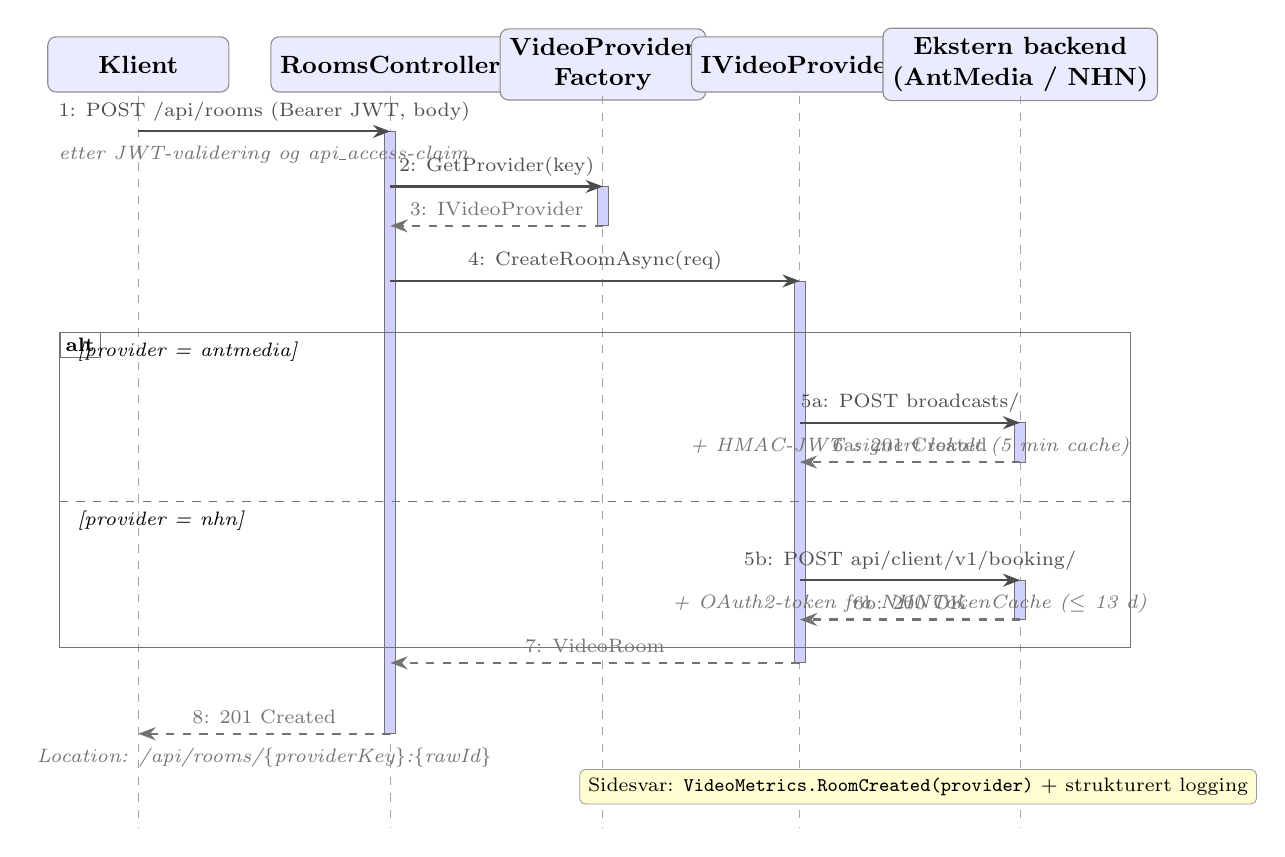
\begin{tikzpicture}[
    >={Stealth[length=2.2mm]},
    actor/.style={
        draw=black!45,
        rounded corners=3pt,
        line width=0.4pt,
        minimum width=2.3cm,
        minimum height=0.7cm,
        fill=blue!8,
        align=center,
        font=\small\bfseries
    },
    msg/.style={->, thick, black!70, font=\footnotesize},
    ret/.style={->, thick, dashed, black!55, font=\footnotesize},
    activ/.style={draw=black!55, fill=blue!18, line width=0.3pt},
    altframe/.style={draw=black!55, line width=0.4pt},
    altlbl/.style={fill=white, draw=black!55, line width=0.3pt, font=\scriptsize\bfseries, inner sep=2pt},
    altsep/.style={dashed, black!55, line width=0.4pt},
    note/.style={draw=black!40, fill=yellow!18, line width=0.3pt, font=\scriptsize, align=left, inner sep=3pt, rounded corners=2pt}
]

% --- Lifeline x-positions ---
\def\xKli{0}
\def\xCtrl{3.2}
\def\xFact{5.9}
\def\xProv{8.4}
\def\xBack{11.2}

% --- Actor headers ---
\node[actor] (kli)  at (\xKli,  0) {Klient};
\node[actor] (ctrl) at (\xCtrl, 0) {RoomsController};
\node[actor] (fact) at (\xFact, 0) {VideoProvider\\Factory};
\node[actor] (prov) at (\xProv, 0) {IVideoProvider};
\node[actor] (back) at (\xBack, 0) {Ekstern backend\\(AntMedia / NHN)};

% --- Lifelines ---
\def\bottomy{-9.7}
\foreach \x in {\xKli,\xCtrl,\xFact,\xProv,\xBack}
    \draw[dashed, black!35] (\x, -0.4) -- (\x, \bottomy);

% --- Activation bars ---
\fill[activ] (\xCtrl-0.07, -0.85) rectangle (\xCtrl+0.07, -8.5);
\fill[activ] (\xFact-0.07, -1.55) rectangle (\xFact+0.07, -2.05);
\fill[activ] (\xProv-0.07, -2.75) rectangle (\xProv+0.07, -7.6);
\fill[activ] (\xBack-0.07, -4.55) rectangle (\xBack+0.07, -5.05);
\fill[activ] (\xBack-0.07, -6.55) rectangle (\xBack+0.07, -7.05);

% --- Messages ---
% 1. Klient -> Controller
\draw[msg] (\xKli, -0.85) -- (\xCtrl, -0.85)
    node[midway, above, font=\scriptsize] {1: POST /api/rooms (Bearer JWT, body)};
\node[font=\scriptsize, black!55] at ($(\xKli, -0.85)!0.5!(\xCtrl, -0.85) + (0,-0.30)$)
    {\textit{etter JWT-validering og api\_access-claim}};

% 2. Controller -> Factory
\draw[msg] (\xCtrl, -1.55) -- (\xFact, -1.55)
    node[midway, above, font=\scriptsize] {2: GetProvider(key)};

% 3. Factory -> Controller (return)
\draw[ret] (\xFact, -2.05) -- (\xCtrl, -2.05)
    node[midway, above, font=\scriptsize] {3: IVideoProvider};

% 4. Controller -> Provider
\draw[msg] (\xCtrl, -2.75) -- (\xProv, -2.75)
    node[midway, above, font=\scriptsize] {4: CreateRoomAsync(req)};

% --- alt fragment ---
\draw[altframe] (\xKli-1.0, -3.4) rectangle (\xBack+1.4, -7.4);
\node[altlbl, anchor=north west] at (\xKli-1.0, -3.4) {alt};

% [antmedia] branch
\node[font=\scriptsize\itshape, anchor=west] at (\xKli-0.9, -3.65) {[provider = antmedia]};

% 5a. Provider -> Backend (AntMedia)
\draw[msg] (\xProv, -4.55) -- (\xBack, -4.55)
    node[midway, above, font=\scriptsize] {5a: POST broadcasts/};
\node[font=\scriptsize, black!55] at ($(\xProv, -4.55)!0.5!(\xBack, -4.55) + (0,-0.30)$)
    {\textit{+ HMAC-JWT signert lokalt (5 min cache)}};

% 6a. Backend -> Provider (return)
\draw[ret] (\xBack, -5.05) -- (\xProv, -5.05)
    node[midway, above, font=\scriptsize] {6a: 201 Created};

% --- separator ---
\draw[altsep] (\xKli-1.0, -5.55) -- (\xBack+1.4, -5.55);
\node[font=\scriptsize\itshape, anchor=west] at (\xKli-0.9, -5.80) {[provider = nhn]};

% 5b. Provider -> Backend (NHN)
\draw[msg] (\xProv, -6.55) -- (\xBack, -6.55)
    node[midway, above, font=\scriptsize] {5b: POST api/client/v1/booking/};
\node[font=\scriptsize, black!55] at ($(\xProv, -6.55)!0.5!(\xBack, -6.55) + (0,-0.30)$)
    {\textit{+ OAuth2-token fra NHNTokenCache ($\le$ 13 d)}};

% 6b. Backend -> Provider (return)
\draw[ret] (\xBack, -7.05) -- (\xProv, -7.05)
    node[midway, above, font=\scriptsize] {6b: 200 OK};

% --- end alt ---

% 7. Provider -> Controller (return)
\draw[ret] (\xProv, -7.6) -- (\xCtrl, -7.6)
    node[midway, above, font=\scriptsize] {7: VideoRoom};

% 8. Controller -> Klient (return)
\draw[ret] (\xCtrl, -8.5) -- (\xKli, -8.5)
    node[midway, above, font=\scriptsize] {8: 201 Created};
\node[font=\scriptsize, black!55] at ($(\xKli, -8.5)!0.5!(\xCtrl, -8.5) + (0,-0.30)$)
    {\textit{Location: /api/rooms/\{providerKey\}:\{rawId\}}};

% --- Side-effect note ---
\node[note, anchor=north west] at (\xFact-0.3, -8.95)
    {Sidesvar: \texttt{VideoMetrics.RoomCreated(provider)} + strukturert logging};

\end{tikzpicture}
\caption{Sekvensdiagram for opprettelse av videorom. Controlleren er provider-agnostisk: \texttt{VideoProviderFactory} løser opp riktig \texttt{IVideoProvider} via keyed dependency injection, og en \texttt{DelegatingHandler} på provider-laget håndterer den backend-spesifikke autentiseringen. \texttt{alt}-fragmentet viser hvor abstraksjonen brytes: AntMedia signerer en kortlevd JWT lokalt (HMAC-SHA256, 5 minutters cache), mens NHN bruker et OAuth2-token fra \texttt{NHNTokenCache} med levetid på inntil 13 dager.}
\label{fig:sekvens-opprette-rom}
\end{figure}
